\documentclass[11pt,a4paper,titlepage]{article}
\usepackage{amsmath}
\usepackage{amssymb}
\usepackage{wasysym}
\usepackage{float}
\usepackage{latexsym,amsmath,amssymb}
\usepackage{graphicx}
\usepackage{epstopdf}
%\usepackage{subfig}
\usepackage{slashed}
\usepackage{bm}
\usepackage{epsfig}
\usepackage{cases}
\usepackage{dcolumn}
\usepackage{color}
\usepackage[colorlinks=true,linkcolor=red]{hyperref}
\usepackage{listings} 
\usepackage{xcolor} % for setting colors
\begin{document}
\begin{titlepage}
%\vspace*{3cm}
\begin{center}
\Huge {A tutorial on gtools to solve Differential Equations} 
\end{center}
\vspace{3cm}
\begin{center}
\Large{gtools (V1.0.0)}
\end{center}
\vspace{2cm} 
\begin{center} 
Mithun Bairagi \\[3pt]  
\textit{Department of Physics, The University of Burdwan, Golapbag 713104, West Bengal, India} \\ [1cm]
%\textit{Address} \\ [1cm] 
\today
\end{center}
\end{titlepage}
 
\clearpage
gtools is a command-line interface for GiNaCDE library. It requires no GUI tools. It is executed in console mode. 
The usage of gtools for solving differential equations is described in this tutorial. The following two examples demonstrate the usage of gtools to solve differential equations.
\section{Example 1}
Let us consider the Eckhaus equation 
\begin{equation}\label{eckhaus}
	i{u_t} + {u_{xx}} + 2{\left( {{{\left| u \right|}^2}} \right)_x}u + {\left| u \right|^4}u = 0.
\end{equation}
For solving Eq. \eqref{eckhaus} using GiNaCDE library, the C++ codes are\\
\begin{verbatim}
// eckhaus_FIM.cpp
#include <GiNaCDE/GiNaCDE.h>
int main()
{
    const ex u=reader("u"), t=reader("t"), x=reader("x"), 
             a=reader("a"), b=reader("b"),k=reader("k");   
    depend(u, {t, x});
    const ex pde = I*Diff(u,t,1) + Diff(u,x,2) + 2*u*Diff(u*conjugate(u),x,1)
                   + u*u*conjugate(u)*conjugate(u)*u;
    output = mathematica;  
    twcPhase=lst{lst{-2*k*a,k},lst{b,a}};
    paraInDiffSolve=lst{};
    filename = "eckhaus_FIM.txt";
    desolve(pde,{u},FIM);
    return 0;
}
\end{verbatim}
In the following, we display the screenshots of each step when we implement the above C++ code in gtools.

\begin{figure}[H]
	\centering
	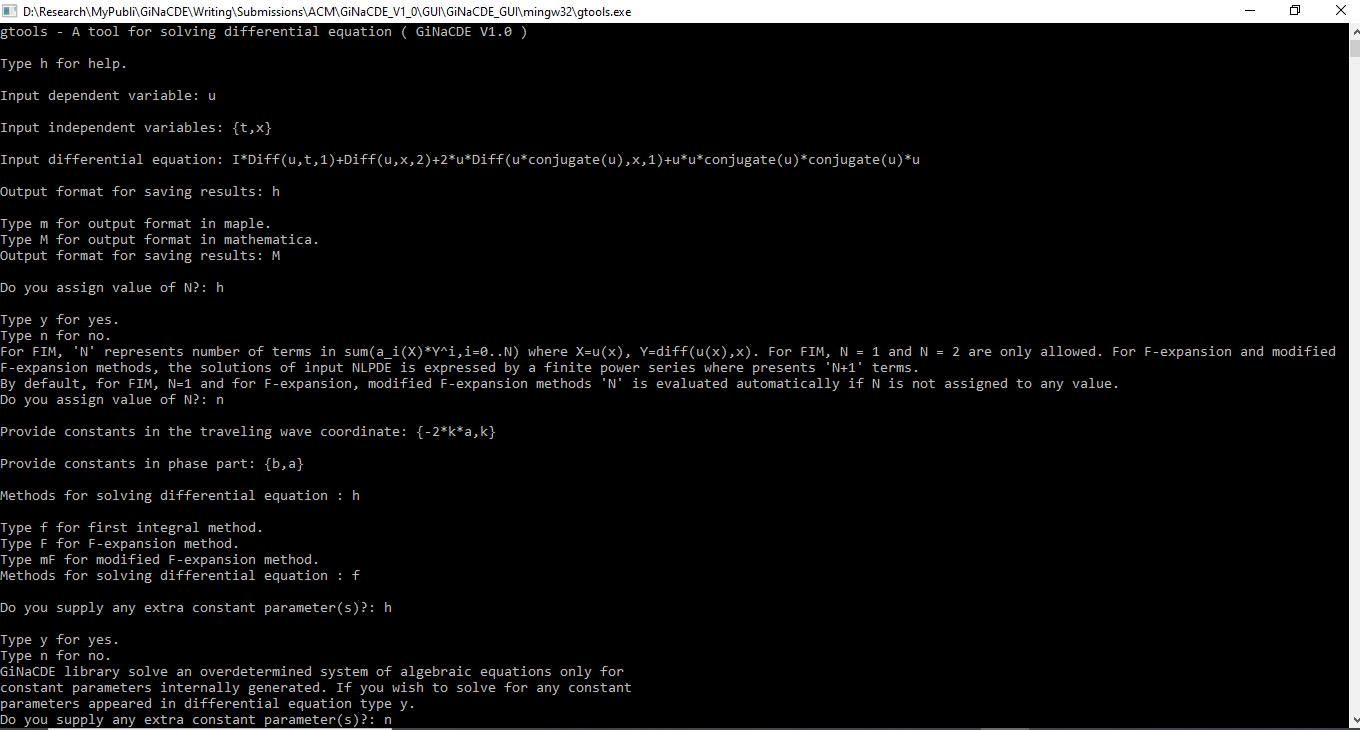
\includegraphics[width=\linewidth]{gtools_ss1}
	\caption{ Screenshot 1. }
	\label{fig:gtools_ss1}
\end{figure}

\begin{figure}[H]
	\centering
	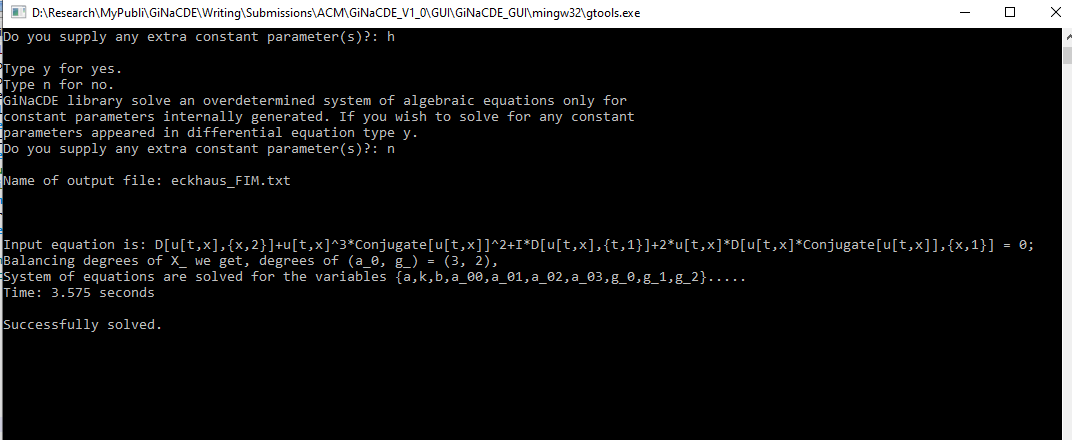
\includegraphics[width=\linewidth]{gtools_ss2}
	\caption{ Screenshot 2. }
	\label{fig:gtools_ss2}
\end{figure}


After execution of the last step in fig. \ref{fig:gtools_ss2} the output results are saved in \emph{eckhaus\_FIM.txt} file.
\section{Example 2}
We now discuss an another example considering generalized Camassa-Holm equation
\begin{equation}\label{Camassa}
	{u_t} + 2k{u_x} - {u_{xxt}} + au{u_x} - 2{u_x}{u_{xx}} - u{u_{xxx}} = 0.
\end{equation}
The following C++ code solve Eq. \eqref{Camassa} applying modified F-expansion method.
\newline
\begin{verbatim}
	// Generalized_Camassa-Holm_mF.cpp
	#include <GiNaCDE/GiNaCDE.h>
	int main()
	{
	    const ex u=reader("u"),t=reader("t"), x=reader("x"), 
	             k=reader("k"), a=reader("a"), k_0=reader("k_0"), 
	             k_1=reader("k_1"), A_1=reader("A_1"),A_3=reader("A_3");   
	    depend(u, {t,x});
	    const ex pde = Diff(u,t,1)+2*k*Diff(u,x,1)-Diff(Diff(u,x,2),t,1)
	                   +a*u*Diff(u,x,1)-2*Diff(u,x,1)*Diff(u,x,2)
	                   -u*Diff(u,x,3); 
	    output = maple;
	    twcPhase = lst{lst{k_0,k_1},lst{}};
	    degAcoeff = lst{3,0,A_1,0,A_3};
	    NValue = 2;
	    filename = "Generalized_Camassa-Holm_mF.txt";
	    ASolve=false;
	    positivePart = true; 
	    negativePart = true;
	    paraInDiffSolve = lst{k,a};
	    desolve(pde, {u}, mF_expansion);
	    return 0;
	}
\end{verbatim}
The following screenshot expresses each step to implement the above C++ code in gtools.


\begin{figure}[H]
	\centering
	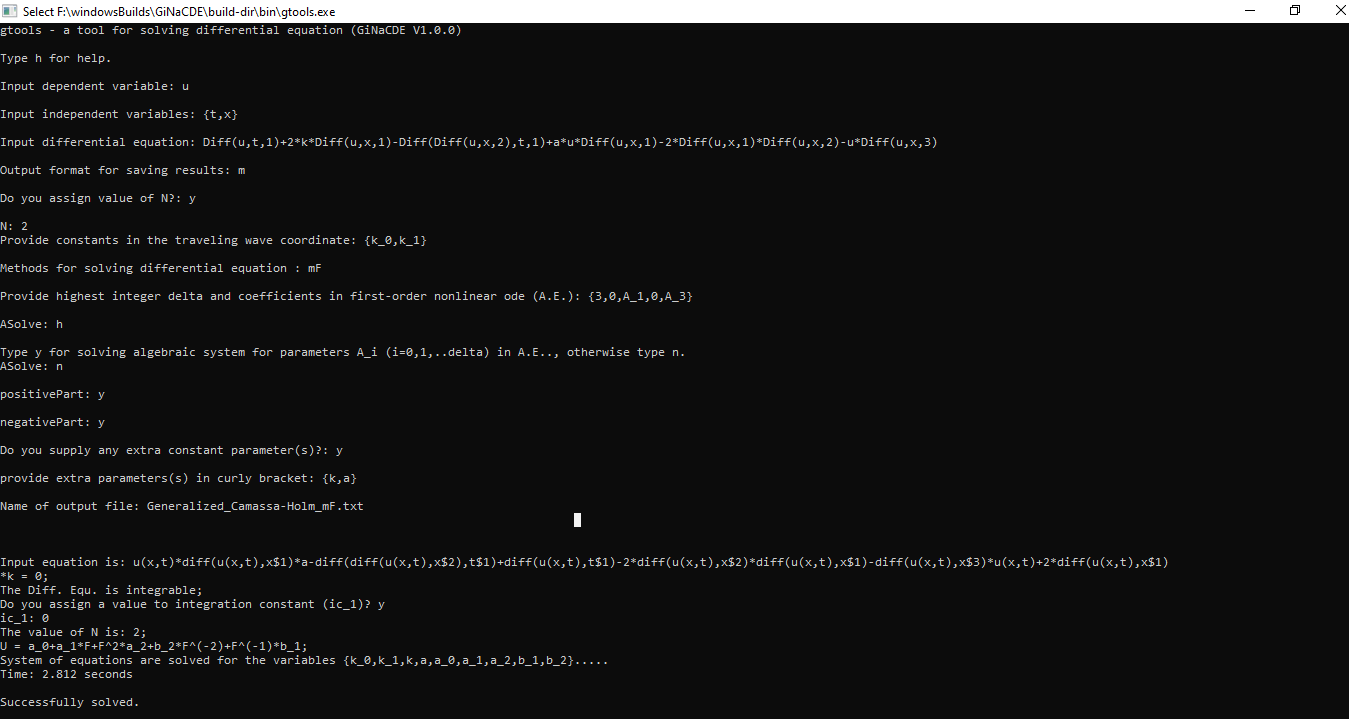
\includegraphics[width=\linewidth]{gtools_ss3}
	\caption{ Screenshot 1. }
	\label{fig:gtools_ss3}
\end{figure}



After execution of the last step in fig. \ref{fig:gtools_ss3} the output results are saved in \emph{Generalized\_Camassa-Holm.txt} file.
\end{document}